%%%%%%%%%%%%%%%%%%%%%%%%%%%%%%%%%%%%%%%%%%%%%%%%%%%%%%%%%%%%%%%%%%%%%%%%%%%%%%%
\section{Future Work}
%%%%%%%%%%%%%%%%%%%%%%%%%%%%%%%%%%%%%%%%%%%%%%%%%%%%%%%%%%%%%%%%%%%%%%%%%%%%%%%

The software library {\tt abelfunctions} provides a collection of tools
for computing on Riemann surfaces. Although more features need to be
added most of the package's functionality is ready to be used to solve
problems. In this section, I present several problems that I wish to
address for my thesis:
\begin{itemize}
  \item Provide solutions to non-linear, integrable, partial
    differential equations.
  \item Provide a framework for constructing and computing rational
    functions on Riemann surfaces with prescribed poles and zeros.
  \item Efficiently compute linear matrix representations of plane
    algebraic curves.
\end{itemize}



%------------------------------------------------------------------------------
\subsection{Solutions to Integrable Partial Differential Equations}
%------------------------------------------------------------------------------



We return to the Kadomtsev--Petviashvili (KP) equation given in the
introductory section of this document:
\begin{equation*}
    \left(-4u_t + 6uu_x + u_{xxx}\right)_x + 3\sigma^2 u_{yy} = 0.
\end{equation*}
As mentioned, the KP equation has a large class of quasi-periodic solutions of
the form
\begin{equation}\label{eqn: solnformula}
    u(x,y,t)
    =
    2 \partial_x^2 \log \theta(Ux + Vy + Wt + z_0, \Omega) + c.
\end{equation}

There is a deep connection between the Riemann matrix appearing in the
second argument of the theta function above and period matrices.
\begin{theorem}
  {\bf (Novikov Conjecture (1965) / Shiota Theorem (1986))}
  \cite{Shiota86} A Riemann matrix $\Omega \in \hh_g$ is a period matrix
  if and only if there exists $U,V,W,z_0 \in \CC^g$ and $c \in \CC$ such
  that
  \[
      u(x,y,t)
      =
      2 \partial_x^2 \log \theta(Ux + Vy + Wt + z_0, \Omega) + c
  \]
  is a solution to the Kadomtsev--Petviashvili equation.
\end{theorem}
That is, the KP equation provides a certification for whether or not a
Riemann matrix is a period matrix. In fact, as the genus $g$ increases
the likelihood that a randomly chosen Riemann matrix is a period matrix
decreases. By a simple counting argument,
\[
    \dim_{\CC} \hh_g = g(g+1)/2.
\]
However,
\[
    \dim_{\CC} \{ \text{period matrices} \} = 3g-3.
\]
For $g=2,3$ the dimensions are equal, implying that every Riemann matrix
is a period matrix. (This is also the case when $g=1$.)  However, for $g
> 3$ the space of Riemann matrices is larger than that of period
matrices.

The main point of this discussion is that the Kadomtsev--Petviashvili
equation plays a very important role in the theory of period matrices
and establishes a very strong link between the fields of complex
algebraic geometry and integrable partial differential equations.

It is possible to compute the constants appearing in Equation
\eqref{eqn: solnformula}. Given a divisor $D = \sum_i n_i P_i$ on $X$
the parameters $U,V,W,z_0 \in \CC^g$ and $c \in \CC$ can be determined
by integrating certain meromorphic differentials around certain paths on
$X$. Deconinck \cite{DS98} provides a method for determining a divisor
from a set of initial data to the KP equation, thus allowing a more
``physical'' input to the solution algorithm. That is, the machinery for
computing solutions of the form above can be used to solve the initial
value problem to KP.

The algorithms and infrastructure needed to define divisors and compute
these quantities is the first problem I plan to address in my thesis
work. Additionally, I will provide a standardized, programmatical
framework for developers to add their own solution formulas to other
integrable partial differential equations. The tools necessary for
computing solutions to KP are the same as those needed to compute the
parameters appearing in other finite genus solution formulas. Therefore,
KP is a logical first step to this objective.

%------------------------------------------------------------------------------
\subsection{The Schottky--Klein Prime Form}
%------------------------------------------------------------------------------


In addition to providing the means of computing paths and 1-forms on a
Riemann surface $X$ it is important to have a way of constructing
functions, other than the Abel map, defined on $X$. For example, is it
possible to construct and subsequently compute meromorphic functions
with prescribed zeros and poles on $X$? That is, does a function $E : X
\times X \to \CC$ exist such that $E(P,Q) = 0$ if and only if $P = Q$?
It turns out that such a function ``almost'' exists yet satisfies enough
properties to make the function useful.

We first need a special class of theta characteristics.
\begin{definition}
  A {\bf non-singular odd theta characteristic} $[\delta] := [\alpha,
    \beta]$ is a theta characteristic where, for a given $\alpha,\beta
  \in \{0,1/2\}^g$,
  \begin{itemize}
    \item $\nabla\theta[\alpha,\beta](0,\Omega) \neq \mathbf{0}$ and
    \item $4 \alpha \cdot \beta \equiv 1 \pmod{2}$.
  \end{itemize}
  A {\bf non-singular even theta characteristic} is a theta
  characteristic where, instead,
  \[
      4 \alpha \cdot \beta \equiv 0 \pmod{2}.
  \]
\end{definition}

With these characteristics in hand, we define the function of interest.
\begin{definition}
  The {\bf Schottky--Klein prime form} $E: X \times X \to \CC$ is defined
  by
  \begin{align*}
    E(P,Q)
    &=
    \frac{
      \theta[\delta]
      \left( \int_{P}^{Q}\mathbf{\omega},\Omega \right)
    }
    {
      \sqrt{\zeta(P)}\sqrt{\zeta(Q)}
    } \\
    &=
    \frac{
      \theta[\delta]
      \left( A(Q) - A(P), \Omega \right)
    }
    {
      \sqrt{\zeta(P)}\sqrt{\zeta(Q)}
    }
  \end{align*}
  where $\omega = (\omega_j)_{j=1}^g$ is the vector of the normalized
  basis of holomorphic 1-forms of $X$, $A: X \to \CC^g$ is the
  Abel--Jacobi map, and for a given non-singular odd theta
  characteristic $[\delta]$
  \begin{align*}
    \zeta(P)
    &= \nabla \theta[\delta](0,\Omega) \cdot \omega(P) \\
    &= \sum_{j=1}^g \frac{\partial}{\partial z_j}
    \theta[\delta](0,\Omega) \omega_j(P).
  \end{align*}
\end{definition}

Unfortunately, $E$ is not holomorphic on $X \times X$ nor is it even
well defined in part because it depends on the choice of path from $P_1$
to $P_2$. However, it is holomorphic and well-defined on $\tilde{X}
\times \tilde{X}$ where $\tilde{X}$ is the universal cover of the
Riemann surface $X$ which, in this case, is the cut surface
$\hat{X}$. The good news is that the zeros of $E$ are independent of the
choice of representative from the universal cover: if
$(\tilde{P}_1,\tilde{Q}_1) \in \tilde{X} \times \tilde{X}$ and
$(\tilde{P}_2,\tilde{Q}_2) \in \tilde{X} \times \tilde{X}$ have the same
projection $(P,Q) \in X \times X$ then $E(\tilde{P}_1,\tilde{Q}_1) = 0$
if and only if $E(\tilde{P}_2,\tilde{Q}_2) = 0$.

As a result, one can use the Schottky--Klein prime form to define
meromorphic functions on a Riemann surface $X$. Let
$P_1,\ldots,P_m,Q_1,\ldots,Q_n \in X$. Then the function
\[
    f : X \to \CC, \quad
    f(P) = \frac{\prod_{i=1}^m E(P,P_i)}{\prod_{j=1}^n E(P,Q_j)}
\]
has zeros at the places $P_1,\ldots,P_m$ and poles at the places
$Q_1,\ldots,Q_n$. The ability to efficiently construct and quickly
evaluate the prime form would make rational functions on Riemann
surfaces as computationally accessible as Abelian functions.

%% \begin{enumerate}
%%   \item $E(P,Q) = 0$ if and only if $\tilde{P} = \tilde{Q}$.
%%   \item $E(P,Q) = - E(Q,P)$.
%%   \item $E$ is invariant under $a$-periods: if
%%     \[
%%     P \mapsto P' = P + \sum m_i A_i
%% \end{enumerate}

%------------------------------------------------------------------------------
\subsection{Linear Matrix Representations}
%------------------------------------------------------------------------------

The Schottky--Klein prime form appears in the construction of linear
matrix representations of certain plane curves. Every complex homogeneous
polynomial in three variables can be written as
\[
    F(x,y,z) = \det \left( Ax + By + Cz \right)
\]
where $A,B,C$ are symmetric matrices \cite{Quarez12}. Such a
representation is called a {\it linear matrix representation}. Linear
matrix representations of polynomials appear in problems in control
theory and can be used to solve polynomial inequalities via semi-definite
programming \cite{HeltonVinnikov07,PSV10}.

The curves we consider here originate from spectrahedra. A {\it
  two-dimensional spectrahedron} is a subset of $\RR^2$ bounded by
rigidly convex algebraic curves; real curves with a maximal number of
nested ovals in the real plane. The interior of the innermost oval of
such a curve defines a spectrahedron. For example, the real projective
curve
\[
    F(x_0,x_1,x_2) =
    2x_0^4 + x_1^4 + x_2^4 - 3x_0^2x_1^2 - 3x_0^2x_2^2 + x_1^2x_2^2,
\]
of degree four with affine part
\[
    f(x,y) = x^{4} + x^{2} y^{2} - 3 x^{2} + y^{4} - 3 y^{2} + 2,
\]
has $4/2 = 2$ nested ovals, as shown in Figure \ref{fig:
  spectrahedron}. These curves are called {\it Helton--Vinnikov curves}
and, by the Helton-Vinnikov theorem, completely characterize all
two-dimensional spectrahedra \cite{HeltonVinnikov07}.

\begin{figure}[t]
  \centering
  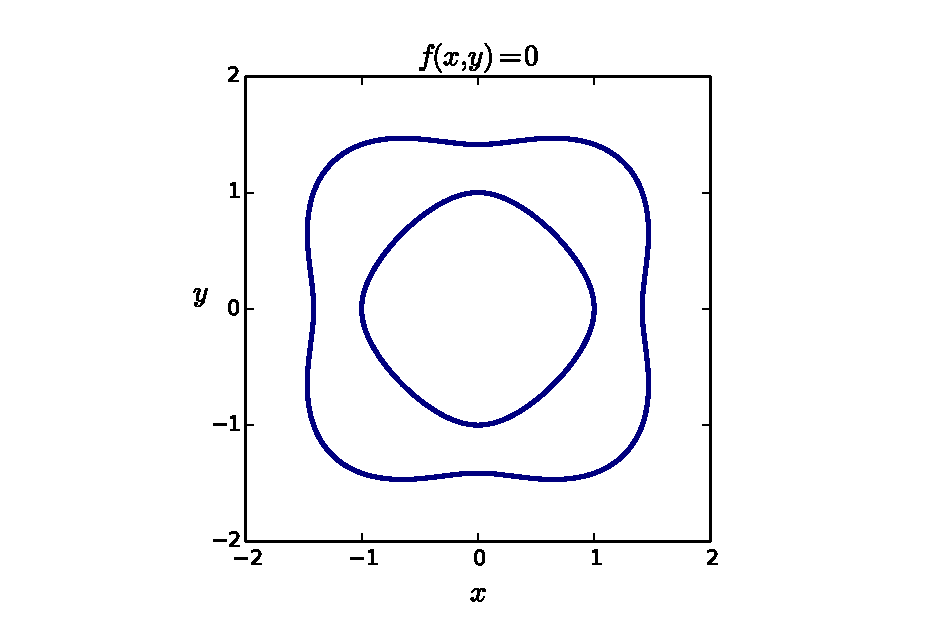
\includegraphics[width=\textwidth]{images/heltonvinnikov.eps}
  \caption{A real plot of the Helton-Vinnikov curve $f(x,y) = x^{4} +
    x^{2} y^{2} - 3 x^{2} + y^{4} - 3 y^{2} + 2$. The region bounded by
    the innermost oval is a spectrahedron.}
  \label{fig: spectrahedron}
\end{figure}

In some applications, it is preferred to have the matrices $A,B,C$ be
real when the curve $F$ is real. The representations important to
studying spectrahedra also require that the linear matrix representation
is a {\it real definite representation}; that is, that the span of
$A,B,$ and $C$ contain a real positive definite matrix. Plaumann,
Sturmfels, and Vinzant \cite{PSV10} study several approaches to
computing real definite matrices of Helton--Vinnikov curves.

The approach chosen by Helton and Vinnikov gives a positive definite
linear matrix representation of a Helton-Vinnikov curve in terms of
theta functions and the Schottky--Klein prime form.

\begin{theorem}
{\bf (Helton--Vinnikov)} Let $C : f(x,y,z) = 0$ be a real homogeneous
curve of degree $d$ with $f(1,0,0) = 0$ and assume
\begin{enumerate}
  \item $C$ is a Helton--Vinnikov curve with the point $f(1,0,0) = 0$
    inside the innermost oval,
  \item the $d$ real intersection points with the line $\{z = 0\}$ are
    distinct non-singular points $Q_1,\ldots,Q_d$ with coordinates $Q_i
    = (-\beta_i : 1 : 0), \beta_i \neq 0$,
  \item $\delta$ is an even theta characteristic with
    $\theta[\delta](0,\Omega) \neq 0$.
\end{enumerate}
Then,
\[
    f(x,y,z) = \det \left( Ix + By + Cz \right),
\]
where $I$ is the $d \times d$ identity matrix, $B =
\text{diag}(\beta_1,\ldots,\beta_d)$, and $C$ is a real symmetric matrix
with diagonal entries
\[
    c_{ii} = \beta_i
    \frac{\partial_z f(-\beta_i,1,0)}{\partial_y f(-\beta_i,1,0)},
\]
and off-diagonal entries
\[
    c_{jk} = \frac{\beta_k - \beta_j}{\theta[\delta](0,\Omega)}
    \frac{\theta[\delta](A(Q_k) - A(Q_j))}{E(Q_j,Q_k)},
\]
where $E : X \times X \to \CC^g$ is the Schottky--Klein prime form.
\end{theorem}

The calculation of linear matrix representations of Helton--Vinnikov
curves is an excellent application of the Schottky--Klein prime form and
I aim to provide an algorithm for doing so.


%------------------------------------------------------------------------------
\subsection{The Constructive Schottky Problem}
%------------------------------------------------------------------------------

As mentioned, the KP equation provides a means for determining if a
Riemann matrix $\Omega \in \hh_g$ comes from the period matrix of some
Riemann surface $X$. The question can be asked, can we find a curve $C :
f(x,y) = 0$ producing this period matrix. This question is called the
Constructive Schottky Problem. That is,
\begin{quote}
  Given a Riemann matrix $\Omega \in \hh_g$ can we find a curve $C :
  f(x,y) = 0$ with $\Omega$ as its period matrix?
\end{quote}
This is a long term endeavor. Regardless, I look to examine possible
avenues for addressing this problem.
